\documentclass{beamer}
\usetheme[nat,greyfoot,footstyle=low,style=alternative,12pt]{Frederiksberg}

\usepackage[utf8]{inputenc} \usepackage{MinionPro} \usepackage{MyriadPro}
\usepackage{graphicx} \usepackage{minted} \usepackage{multicol}
\usepackage{listings} \usepackage{xcolor}

\newcommand{\backupbegin}{
   \newcounter{finalframe}
   \setcounter{finalframe}{\value{framenumber}}
}
\newcommand{\backupend}{
   \setcounter{framenumber}{\value{finalframe}}
}


\usepackage{tikz}

% Define some colors
\definecolor{mblue}{RGB}{0,0,200}
\definecolor{mred}{RGB}{200,40,0}
\definecolor{mgreen}{RGB}{0,180,0}
\definecolor{mdarkgreen}{RGB}{0,100,0}
\definecolor{morange}{RGB}{200,100,0}

\definecolor{lightblue}{RGB}{197,227,240}
\definecolor{lightgreen}{RGB}{197,240,184}

\definecolor{scopebg}{RGB}{250,250,250}
\definecolor{scopeborder}{RGB}{200,200,200}

\usetikzlibrary{calc}
\usetikzlibrary{positioning}
\usetikzlibrary{arrows.meta}
\usetikzlibrary{shapes}
\usetikzlibrary{matrix}
\usetikzlibrary{fit}
\usetikzlibrary{patterns}
\usetikzlibrary{backgrounds}
\usetikzlibrary{decorations.pathreplacing}

\lstdefinelanguage{smeil}
{
  morekeywords={
    as,
    assert,
    async,
    barrier,
    break,
    bus,
    case,
    const,
    default,
    elif,
    else,
    enum,
    exposed,
    for,
    from,
    func,
    generate,
    if,
    import,
    in,
    instance,
    network,
    of,
    out,
    proc,
    range,
    return,
    simulation,
    switch,
    sync,
    to,
    trace,
    unique,
    var
  },
  sensitive=true,
  morecomment=[l]{//},
  morestring=[b]''
}
\lstset{
  columns=fixed,
  %basicstyle=\ttfamily\bfseries\small,
  basicstyle=\tiny\fontfamily{pcr}\selectfont,
  emphstyle=,
  %keywordstyle=,
  numbers=none,
  firstnumber=auto,
  identifierstyle=,
  commentstyle=,
  stringstyle=,
  showstringspaces=false,
  captionpos=b,
  xleftmargin=16pt,
  escapeinside={??}
}

\AtBeginSection[]{
  \begin{frame}[plain,noframenumbering]
  \vfill
  \centering
  \begin{beamercolorbox}[sep=8pt,center,shadow=true,rounded=true]{title}
    \usebeamerfont{title}\insertsectionhead\par%
  \end{beamercolorbox}
  \vfill
  \end{frame}
}


\title{Master's thesis defense}
\subtitle{A Domain Specific Language for Synchronous Message \mbox{Exchange} Networks}
\author{Truls Asheim --- \texttt{truls@asheim.dk}}
\institute{Niels Bohr Institute, University of Copenhagen}
\date{June 18, 2018}

\begin{document}
\maketitle

\section{Introduction}
% \begin{frame}{Outline}
%   \begin{enumerate}
%   \item 
%     \item Live demo!
%   \end{enumerate}
% \end{frame}  

% \begin{frame}
%   \begin{enumerate}
%   \item 
%     \item Live demo!
%   \end{enumerate}
% \end{frame}  

\begin{frame}
  \frametitle{Current tendencies}
  \framesubtitle{Stagnant per-core CPU performance}
    \begin{figure}
      \centering
      \includegraphics[width=0.9\textwidth]{figures/42-years-processor-trend.png}
    \end{figure}
    Parallelism must be exploited in order to achieve performance
    improvements.
  \end{frame}
  % }
  %  \only<2>{

    \begin{frame}
  \frametitle{Current tendencies}
  \framesubtitle{Increasing data center power consumption}
      \begin{figure}
      \centering
      \includegraphics[width=0.8\textwidth]{figures/power_usage.png}
    \end{figure}
    Increased efficiency is needed\footnote{\tiny From: The Internet: Explaining
      ICT Service Demand in Light of Cloud Computing Technologies by Hans Jakob
      Walnum and Anders S.G. Andrae}
    
  %}
  %  \only<3>{
  \end{frame}

%   \begin{frame}[allowframebreaks]{Computational devices}
%     \begin{itemize}
%     \item CPU
%       \begin{itemize}
%       \item Easy to program
%       \item Cheap
%       \item Versatility over performance. Therefore slow and inefficient.
%       \end{itemize}
%     \item GPGPU
%       \begin{itemize}
%       \item Hard to program (but programming tools are becoming quite mature)
%       \item Still quite cheap
%       \item fast and reasonably efficient (for SIMD operations)
%       \end{itemize}
%       \framebreak
%     \item Application-Specific integrated Circuit (ASIC)
%       \begin{itemize}
%       \item Extremely expensive. Infeasible unless a large amount of ICs are
%         needed
%       \item Difficult, slow and work-intensive to develop
%       \item As fast and efficient as you want
%       \end{itemize}
%     \item Field Programmable Gate Array (FPGA)
%       \begin{itemize}
%       \item Compromise between ASICs and general-purpose (GPU and CPU)
%       \item Good performance, better efficiency than GPUs
%       \item Very difficult to program and mature high-level approaches are
%         \begin{itemize}
%         \item difficult to use
%         \item significantly underperforms compared to hand-written designs
%         \end{itemize}
%       \end{itemize}
%     \end{itemize}
%   %}
% \end{frame}

% \begin{frame}
%   Conclusion: Better tools are needed to 
  
% \end{frame}

  \begin{frame}{Custom hardware}
    \begin{itemize}
    \item CPUs are slow and inefficient due to their versatility
    \item GPGPUs achieve significantly better performance and efficiency for
      SIMD workloads
    \item Field-Programmable Gate Arrays (FPGAs) offer good performance, while
      maintaining a much higher efficiency than GPGPUs and especially CPUs. But,
      extremely difficult to program.
    \end{itemize}
    \pause
    \begin{block}{}
      The utilization of FPGAs is being held back (partially) by poor design
      tools and languages. SME was introduced to alleviate this.
    \end{block}
  \end{frame}
  
\begin{frame}{The Synchronous Message Exchange Model}
  Pure CSP was found to be unfit for modeling hardware due to the overhead
  induced by enforcing global synchrony by modeling a clock.

  \begin{itemize}
    \item SME properties:
  \begin{itemize}
  \item Globally synchronous message propagation
  \item Implicit clock
  \item Shared-nothing
  \end{itemize}
  \item Implementations for Python$\dagger$, C\#$\dagger$, C++
  \item Key features:
  \begin{itemize}
  \item Explicit concurrency using a model mimicking signal propagation in hardware
  \item Allows cycle-accurate simulation of the resulting hardware
  \item Automatic generation of VHDL (from $\dagger$), test bench and test vectors for
    continuous verification of hardware description
  \end{itemize}
  \end{itemize}
  
\end{frame}

\begin{frame}{SME Workflow}
\begin{figure}
  \centering
  \resizebox{\linewidth}{!}{
    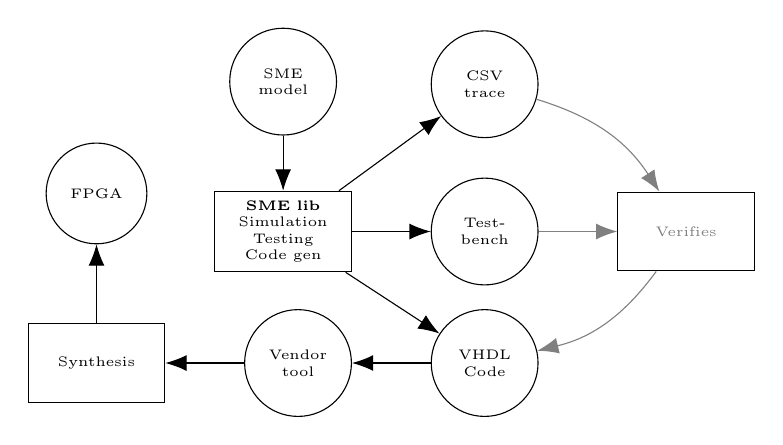
\begin{tikzpicture}[font=\tiny,
      rep style/.style={rectangle,draw=black,text width=1.5cm,minimum
        size=1cm,align=center},
      proc style/.style={circle,draw=black,align=center,text
        width=1cm,minimum size=1cm,align=center}
      ]
      \node[proc style] (impl) {SME model};
      \node[rep style,below=0.7cm of impl] (sim) {{\bfseries SME
        lib}\\Simulation\\Testing\\Code gen};
      \node[proc style,right=1cm of sim] (tb) {Test-bench};
      \node[proc style,above=0.5cm of tb] (trace) {CSV trace};
      \node[proc style,below=0.3cm of tb] (code) {VHDL Code};
      \node[gray,draw=gray,rep style,right=1cm of tb] (verifies) {Verifies};
      \node[proc style,left=1cm of code] (vendor) {Vendor tool};
      \node[rep style,left=1cm of vendor] (synth) {Synthesis};
      \node[proc style,above=1cm of synth] (fpga) {FPGA};


      \draw[-{Latex[scale=1.6]}] (impl) edge [] (sim);
      \draw[-{Latex[scale=1.6]}] (sim) edge [] (trace);
      \draw[-{Latex[scale=1.6]}] (sim) edge [] (tb);
      \draw[-{Latex[scale=1.6]}] (sim) edge [] (code);

     \draw[-{Latex[scale=1.6]}] (trace) edge [gray, bend left=20] (verifies);
     \draw[-{Latex[scale=1.6]}] (tb) edge [gray] (verifies);
     \draw[-{Latex[scale=1.6]}] (verifies) edge [gray, bend left=20] (code);

     \draw[-{Latex[scale=1.6]}] (code) edge [] (vendor);
     \draw[-{Latex[scale=1.6]}] (vendor) edge [] (synth);
     \draw[-{Latex[scale=1.6]}] (synth) edge [] (fpga);

    \end{tikzpicture}}
\end{figure}

\end{frame}

\begin{frame}{Initial motivation}
  \begin{block}{Challenges}
  \begin{itemize}
  \item Most SME development focused on C\#, though the SME model was not
    intended to be specific to a single language. Thus, wider language support
    was desirable.
  %\item Most SME 
  \item Maintaining feature-parity of several independent SME implementations is
    infeasible due to duplication of code and effort.
  \item Interaction between SME components written using SME implementations for
    different languages was not possible.
  \end{itemize}
\end{block}

  \pause

  \begin{block}{Solution}
    Introducing a common intermediate language and common tooling for the SME
    model.
  \end{block}

\end{frame}

\begin{frame}{Initial motivation: Common IL}
  \noindent\begin{minipage}[t]{.5\linewidth}
   % \begin{center}
  \resizebox{0.\linewidth}{!}{
    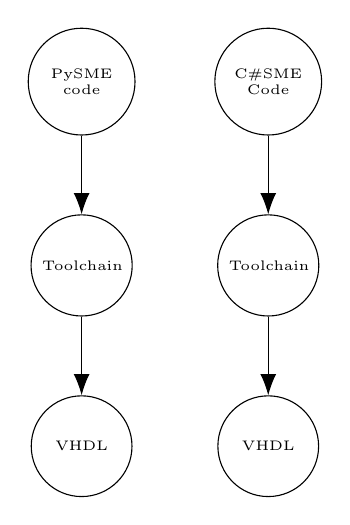
\begin{tikzpicture}[font=\tiny,
      rep style/.style={rectangle,draw=black,text width=1.5cm,minimum
        size=1cm,align=center},
      proc style/.style={circle,draw=black,align=center,text
        width=1cm,minimum size=1cm,align=center}
      ]
      
      \node[proc style] (pysme) {PySME code};
      \node[proc style, below=1cm of pysme] (pysmetrans) {Toolchain};
      \node[proc style, below=1cm of pysmetrans] (pysmevhdl) {VHDL};

      \draw[-{Latex[scale=1.6]}] (pysme) edge [] (pysmetrans);
      \draw[-{Latex[scale=1.6]}] (pysmetrans) edge [] (pysmevhdl);

      \node[proc style, right=1cm of pysme] (csme) {C\#SME Code};
      \node[proc style, below=1cm of csme] (csmetrans) {Toolchain};
      \node[proc style, below=1cm of csmetrans] (csmevhdl) {VHDL};

      \draw[-{Latex[scale=1.6]}] (csme) edge [] (csmetrans);
      \draw[-{Latex[scale=1.6]}] (csmetrans) edge [] (csmevhdl);

    \end{tikzpicture}}
  \begin{center}
  Current
\end{center}
\pause
\end{minipage}\hfill
  \begin{minipage}[t]{.49\linewidth}

    \resizebox{0.9\linewidth}{!}{
    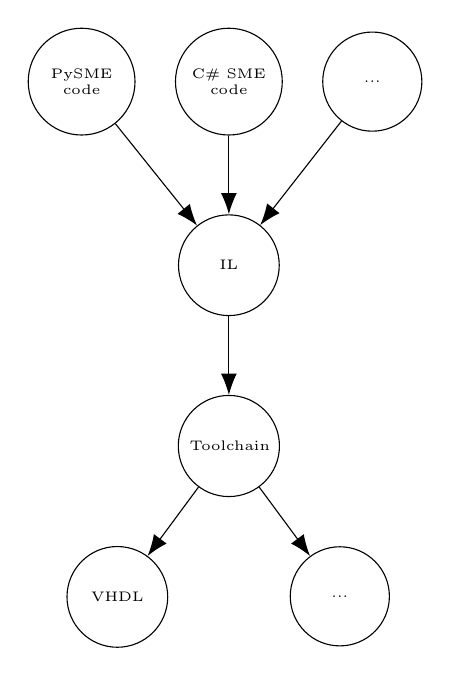
\begin{tikzpicture}[font=\tiny,
      rep style/.style={rectangle,draw=black,text width=1.5cm,minimum
        size=1cm,align=center},
      proc style/.style={circle,draw=black,align=center,text
        width=1cm,minimum size=1cm,align=center}
      ]
      
      \node[proc style] (csme) {C\# SME code};
      \node[proc style, left=0.5cm of csme] (pysme) {PySME code};
      \node[proc style, right=0.5cm of csme] (cother) {...};

      \node[proc style, below=1cm of csme] (smeil) {IL};

      \draw[-{Latex[scale=1.6]}] (pysme) edge [] (smeil);
      \draw[-{Latex[scale=1.6]}] (csme) edge [] (smeil);
      \draw[-{Latex[scale=1.6]}] (cother) edge [] (smeil);
      
      \node[proc style, below=1cm of smeil] (smeilcomp) {Toolchain};

      \node[proc style, below left=1cm and 0.5cm of smeilcomp] (vhdlcomp) {VHDL};
      \node[proc style, below right=1cm and 0.5cm of smeilcomp] (othercomp) {...};

      \draw[-{Latex[scale=1.6]}] (smeil) edge [] (smeilcomp);
      %\draw[-{Latex[scale=1.6]}] (csme) edge [] (csmetrans);
      \draw[-{Latex[scale=1.6]}] (smeilcomp) edge [] (vhdlcomp);
      \draw[-{Latex[scale=1.6]}] (smeilcomp) edge [] (othercomp);

    \end{tikzpicture}}
  \begin{center}Desired
  \end{center}
\end{minipage}


\end{frame}

% \begin{frame}{Contributions}
%   \begin{itemize}
%   \item SMEIL
%   \item Co-simulation
%   \item Observation based typing
%   \item Implementation of above
%   \end{itemize}
% \end{frame}


\section{The SME Implementation Language (SMEIL)}
\begin{frame}{The SMEIL language}
  \begin{itemize}
  \item SME primitives as first-class constructs
    %\pause
  \item Statically checked bit-precise typing
    %\pause
  \item Intentional commonality with general-purpose languages (e.g. Python and
    C\#) (enable straight-forward mapping from high-level languages)
    %\pause
  \item C-like syntax --- A tradeoff between simplicity of parsing and
    readability
    %\pause
  \item Purely a hardware modeling language --- no simulation-only
    features\footnote{Some exceptions}.
  \end{itemize}

  \pause
  \begin{block}{}
  Usable both as a primary implementation language for SME models and as an IL
  for other SME implementations.
\end{block}
\end{frame}

\begin{frame}[fragile]{Example: the addone network}
  %\only<2>{
  \begin{multicols}{2}
\begin{lstlisting}[language=smeil]
proc id(in inbus)
  bus idout {
    val: int = 0;
  };
  var it: uint = 0;
{
  idout.val = inbus.val;
  trace("Iteration: {} Value: {}",
    it, inbus.val);
  it = it + 1;

}




proc incr_const(in inbus, const val)
  bus addout {
    val: int = 0;
  };
{
  addout.val = inbus.val + val;
}

network addone() {
  instance addone_inst of
    incr_const(id_inst.idout, val: 10);
  instance id_inst of
    id(addone_inst.addout);
}
\end{lstlisting}
  \end{multicols}
%}
  %\only<1>{

\begin{figure}
  \resizebox{.6\linewidth}{!}{
    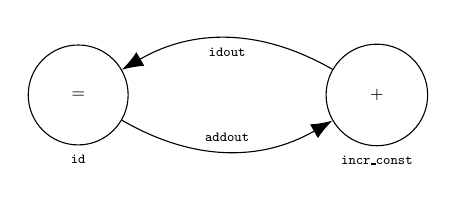
\begin{tikzpicture}[font=\tiny,
      proc style/.style={circle,draw=black,align=center,text
        width=1cm,minimum size=1cm,align=center}
      ]
      \node[proc style] (id) {$=$};
      \node[below=0cm of id] (p1) {{\tt id}};
      \node[proc style,right=2.5cm of id] (add) {$+$};
      \node[below=0cm of add] (p2) {{\tt incr\_const}};
      \draw[-{Latex[scale=1.6]}] (id) edge [bend right=30] node [above] {{\tt addout}} (add);
      \draw[-{Latex[scale=1.6]}] (add) edge [bend right=30] node [below] {{\tt
          idout}}
      (id);
    \end{tikzpicture}
    }%}
\end{figure}
\end{frame}

% \begin{frame}{Possible workflows}
%   \includegraphics[width=\textwidth]{workflows.pdf}
% \end{frame}

\begin{frame}{Supported types}
  \begin{tabular}{l|l}
    \texttt{int}, \texttt{uint} & Unconstrained (unlimited size) signed/unsigned integer\\
    \texttt{i4}, \texttt{u54} &  Constrained signed/unsigned integers \\
    \texttt{bool} & Booleans \\
    \texttt{f32}, \texttt{i64} & Single/double floats\footnote{Currently only for
                                 simulation}\\
    Arrays & Static length non-nested arrays 
  \end{tabular}
\end{frame}

% \begin{frame}{Network composition}
%   TODO: Should this be here? Mention different ways of composing a network
% \end{frame}
\section{Co-simulation}

\begin{frame}{Co-simulation}

  \begin{block}{Why?}
    \begin{itemize}
    \item SMEIL is purely intended for expressing hardware models --- not for
      test benches. Thus, no support for, e.g., file I/O or advanced
      visualization
    \item Therefore: method for providing external interactions is needed
      \end{itemize}
    \end{block}
  \pause
\begin{block}{}
  Key goal: providing seamless integration of SME networks written in SMEIL and
  another language enabling them to be co-simulated as single entity
\end{block}
\end{frame}

\begin{frame}{Co-simulation  (continued)}

\begin{block}{How?}
  Exposing a co-simulation API from libsme enabling external access to
  simulation control and reading/writing from/to bus channels
\end{block}

\pause 
\begin{block}{}
  Co-simulation is a commonly use technique for supplying test vector to
  hardware design (e.g., CoCoTB, VPI, VHPI). The advantage of the SMEIL approach
  is that SME is used on both sides of the co-simulation
\end{block}
\end{frame}


\begin{frame}{Co-Simulation with PySME}
  PySME extended with co-simulation support:

  \includegraphics[width=\textwidth]{co-simulation.pdf}
  \begin{itemize}
  \item Interaction with the SMEIL simulator through a C-API
  \item Exchanged values recorded in trace file for use with VHDL test bench
\end{itemize}
\end{frame}

\begin{frame}[fragile]{PySME co-simulation interface}
  Simple interface enables co-simulation with minimal intrusion on PySME code

  \begin{columns}
    \begin{column}[T]{0.5\textwidth}
      \centering
      Python side
\begin{lstlisting}[language=python]
?{\color{red}{@extends("collector.sme",}}?
        ?{\color{red}{["-f", "--trace", "trace.csv"])}}?
class ColorBin(Network):
  def wire(self, result):
     img_out_data =\
        ?{\color{red}{ExternalBus}}?("image_input")
     result_bus =\
        ?{\color{red}{ExternalBus}}?("bin_count_out")
     self.add(img_out_data)
     self.add(result_bus)
\end{lstlisting}
    \end{column}
    \begin{column}[T]{0.5\textwidth}
      \centering
      SMEIL side
      \begin{lstlisting}[language=smeil]
proc collector (in image_input)
  exposed bus bin_count_out {
     valid: bool;

     low: u32;
      med: u32;
      high: u32;
  };
// [..]
network coll_net() {
  exposed bus image_input {
    valid: bool;
    last_pixel: bool;

     R: u8;
     G: u8;
     B: u8;
};
// [..]
\end{lstlisting}
    \end{column}
  \end{columns}
\end{frame}

% \begin{frame}{Deciding signal widths}
%   \begin{itemize}
%   \item Programs may start out with only unspecified widths
%   \item Then 
%   \item Accurate wire widths derived from simulation input
%   \item Future work: Inferring bus widths through range analysis.
%   \end{itemize}
% \end{frame}

\section{Constraining bit-widths from value observations}

\begin{frame}[shrink]{Constraining bit-widths from value observations}

  \begin{itemize}
  \item Unconstrained integers are not representable in hardware, so
    unconstrained types (e.g. {\tt int}) must be constrained (e.g. {\tt i8})
    before we can generate a hardware description
  \item No registers of pre-defined sizes (bit-widths) exists in hardware, so we
    are free to define the sizes we need
  \item Synthesizing unnecessarily wide wires will lead to wasted space and an
    inefficient implementation
  \item But, knowing the minimal number of bits needed for a value in advance is
    sometimes hard
  \item Most existing hardware description languages either require
    explicit sizing of all integer types or use bad defaults (e.g. an {\tt int}
    is 32-bits)
  \end{itemize}
  \pause
  \begin{block}{Idea}
    Constrain unconstrained channels based on the range of values assigned to
    them during simulation
  \end{block}
\end{frame}

\begin{frame}[fragile]{Example}
Our example from before. Note the unconstrained integer types.
\begin{lstlisting}[language=smeil]
proc id(in inbus)
    bus idout {
        val: ?{\textcolor{red}{\bfseries\underline{int}}}? = 0;
    };
    var it: ?{\textcolor{red}{\bfseries\underline{uint}}}? = 0;
{
    idout.val = inbus.val;
    trace("Iteration: {} Value: {}",
        it, inbus.val);
    it = it + 1;

}

proc incr_const(in inbus, const val)
    bus addout {
       val: ?{\textcolor{red}{\bfseries\underline{int}}}? = 0;
    };
{
    addout.val = inbus.val + val;
}

network addone() {
    instance plusone_inst of incr_const(id_inst.idout, val: 1);
    instance id_inst of id(plusone_inst.addout);
}

\end{lstlisting}


  Lets simulate it for 10 cycles.
\end{frame}

\begin{frame}[fragile]
  Output from simulator after simulation for 10 cycles
\begin{lstlisting}[language=smeil]
proc id (in inbus)
    var it: ?{\textcolor{red}{\bfseries\underline{u6 = 0 range 0 to 10}}}?;
    bus idout {val: ?{\textcolor{red}{\bfseries\underline{i4 = 0 range 0 to 5}}}?;};
{
    idout.val = inbus.val;
    trace("Iteration: {} Value: {}", it, inbus.val);
    it = it + 1;
}

proc plusone (in inbus, const val)
    bus plusout { val: ?{\textcolor{red}{{\bfseries\underline{i4 = 0 range 0 to 5}}}?;};
{
    plusout.val = inbus.val + val;
}

network plusone_net ()
{
    instance id_inst of id(plusone_inst.addout);
    instance plusone_inst of plusone(id_inst.idout, val: 1);
}

\end{lstlisting}
  
  What about 50 cycles?


  
\end{frame}

\begin{frame}[fragile]
  Simulation for 50 cycles:

\begin{lstlisting}[language=smeil]
proc id (in inbus)
    var it: ?{\textcolor{red}{\bfseries\underline{u6 = 0 range 0 to 50}}}?;
    bus idout {val: ?{\textcolor{red}{\bfseries\underline{i6 = 0 range 0 to 25}}}?;};
{
    idout.val = inbus.val;
    trace("Iteration: {} Value: {}", it, inbus.val);
    it = it + 1;
}

proc plusone (in inbus, const val)
    bus plusout { val: ?{\textcolor{red}{{\bfseries\underline{i6 = 0 range 0 to 25}}}?;};
{
    plusout.val = inbus.val + val;
}

network plusone_net ()
{
    instance id_inst of id(plusone_inst.addout);
    instance plusone_inst of plusone(id_inst.idout, val: 1);
}

\end{lstlisting}
  Note: Signedness of original type is  preserved
\end{frame}

\begin{frame}{Usage of observed ranges}

  The SMEIL code with observed ranges has two possible uses:
  \begin{enumerate}
  \item The observed ranges are used for constraining unbounded types in SMEIL
    such that VHDL with bounded types can be generated
    \pause
  \item The original SMEIL code is rewritten to include the updated ranges --
    may be used as input for formal verification.
  \end{enumerate}
\end{frame}

\begin{frame}{New feature: improved range granularity}
  \figureversion{lining}
  \begin{itemize}
  \item In the handed-in version of libsme, all observed ranges was between 0
    and the maximum absolute value
  \item Sufficient for deriving type bounds
  \item However, formal verification of observer ranges required more detail
  \item Therefore, the actual range (e.g. 10 to 55 or -24 to 30) is now tracked
  \item Non-trivial implementation: Added distinction between undefined and
    defined values
  \end{itemize}
  
\end{frame}

\begin{frame}{Evaluation}
  SMEIL has been evaluated through the following examples
  \begin{itemize}
    \item Modification of the PySME to VHDL compiler to generate SMEIL instead of
      VHDL directly
    \item An image pixel color intensity bin counter
    \item \textbf{The core of a high-frequency trading chip} (up next)
    \item An MD5 bruteforcer
    \item A model 7-segment digital clock
  \end{itemize}
  
\end{frame}

% \begin{frame}{Example: Moving averages}
%   \includegraphics[width=\textwidth]{ewmasmenet.pdf}
% \end{frame}

\begin{frame}{Example: High-frequency trading chip}

  Makes a trading decision based on calculation of Exponential Moving Averages with
  long and short decays
  
  \begin{figure}%[tb]
  \centering
  \resizebox{.9\linewidth}{!}{
    \begin{tikzpicture}[font=\small,
      rep style/.style={rectangle,draw=black,text width=1.5cm,minimum
        size=1.5cm,align=center},
      proc style/.style={ellipse,draw=black,align=center,text
        width=1.5cm,minimum size=1.5cm,align=center},
      file style/.style={ellipse,draw=none,align=center,text
        width=1.5cm,minimum size=0.5cm,align=center},
      plot/.pic={
        \node[] (m1) {\includegraphics[width=.25\textwidth]{../figures/ewma-plot.pdf}};
      }
      ]
    
      \node[proc style] (gen) {Data \\ Generator};
      \node[proc style, right=2cm of gen] (long) {Short Decay};
      \node[proc style, below=0.5cm of long] (short) {Long Decay};
      \node[proc style, below right=0cm and 1.5cm of long] (merge) {Merger};

      \node[proc style, below=0.5cm of gen] (sink) {Plotter};

      \pic[local bounding box=plot, above left=0cm and 2cm of sink] {plot};
      
      \draw[-{Latex[scale=1.6]}] (gen) edge (long);
      \draw[-{Latex[scale=1.6]}] (gen) edge (short);
      \draw[-{Latex[scale=1.6]}] (long) edge (merge);
      \draw[-{Latex[scale=1.6]}] (short) edge (merge);
      \draw[-{Latex[scale=1.6]}] (sink) edge (plot);

      % \draw[-{Latex[scale=1.6]}] (gen) edge (collector);

      \draw[-{Latex[scale=1.6]}] (merge) edge [bend left=50] (sink);
      
      \begin{scope}[on background layer]
        \node[draw=scopeborder,fill=scopebg,inner sep=10pt,rounded corners=10pt,anchor=north west,fit=(long)(short)(merge),label={above}:SMEIL] (SMEIL) {};
        \node[draw=scopeborder,fill=scopebg,inner sep=10pt,rounded corners=10pt,anchor=north west,fit=(gen)(sink),label={above}:PySME] (pysme) {};
      \end{scope}
    \end{tikzpicture}
  }

\end{figure}

Uses the co-simulation interface for writing input generation- and verification
code in Python and the core processes in SMEIL

\end{frame}

\begin{frame}{Example: High-frequency trading chip (continued)}
  Result of execution:
  \begin{figure}
  \includegraphics[width=\textwidth]{ewma_plot.pdf}
\end{figure}
\end{frame}

\begin{frame}{Future work}
  \begin{itemize}
    \item Feature parity between SMEIL/libsme and C\# SME: Make SMEIL fully
      capable IL for C\# SME
    \item Hardware-software co-design. Add automatically configured opaque
      interfaces enabling inter-device communication (e.g. between SME processes
      running on GPGPUs and FPGAs)
    \item Formal verification of observationally derived value ranges (in
      progress).
    \item Parameterized network orchestration
    \item Sugary SMEIL: Further improvements of the language as a primary
      implementation language for SME networks
  \end{itemize}
\end{frame}

\begin{frame}{Conclusions}
  \begin{itemize}
  \item We have introduced SMEIL, a DSL for SME networks shown in practice to be
    able represent several designs already implemented in SME

  \item SMEIL is usable both as an intermediate language and as a primary
    implementation language for SME networks
  
  \item Implementation supporting VHDL code generation

  \item Co-simulation interface enabling writing of test code in a
    general-purpose language

  \item The size of values can be constrained based on ranges observed during
    simulation
    
  % \item Multiple workflows: Works both as an intermediate language
  %   (``self-contained'' VHDL generation with trace file) and as an independent
  %   DSL co-simulated with another language.
  \end{itemize}

  \textbf{Questions?}
\end{frame}

% \begin{frame}
%   Thank you!

%   Source code available from \url{https://github.com/truls/libsme}
 
% \end{frame}

\appendix

\backupbegin

\begin{frame}{Implementation}
  \begin{figure}%[tb]
  \centering
  \resizebox{\linewidth}{!}{
    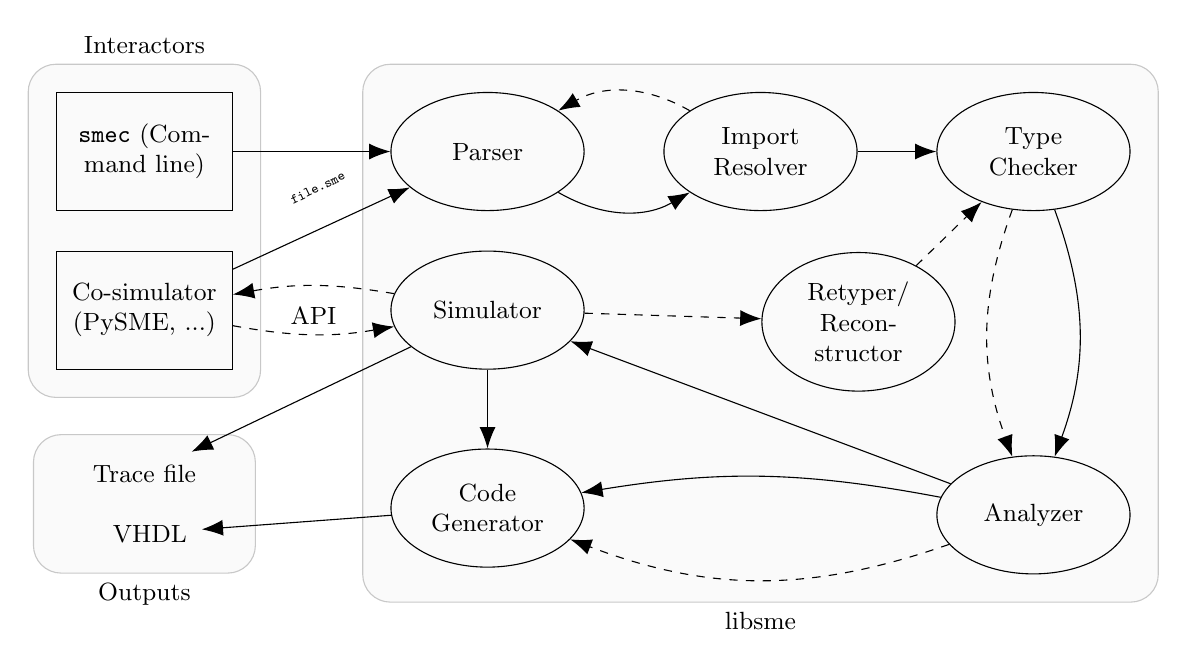
\begin{tikzpicture}[font=\small,
      rep style/.style={rectangle,draw=black,text width=1.5cm,minimum
        size=1.5cm,align=center},
      proc style/.style={ellipse,draw=black,align=center,text
        width=1.5cm,minimum size=1.5cm,align=center},
      file style/.style={ellipse,draw=none,align=center,text
        width=1.5cm,minimum size=0.5cm,align=center}
      ]
      \node[proc style] (parser) {Parser};
      \node[proc style, right=1cm of parser] (import) {Import Resolver};
      \draw[-{Latex[scale=1.6]}] (parser) edge [bend right=30] (import);
      \draw[-{Latex[scale=1.6]},dashed] (import) edge [bend right=30] (parser);

      \node[proc style, right=1cm of import] (tyc) {Type Checker};
      \draw[-{Latex[scale=1.6]}] (import) edge (tyc);
      \node[proc style, below=3.1cm of tyc] (an) {Analyzer};

      \draw[-{Latex[scale=1.6]}] (tyc) edge [bend left=20] (an);
      \draw[-{Latex[scale=1.6]},dashed] (tyc) edge [bend right=20] (an);

      \node[proc style, below right=1cm and -0.5cm of import] (recon) {Retyper/\\Recon-\\structor};
      \node[proc style, below=0.5cm of parser] (sim) {Simulator};
      \node[proc style, below=1cm of sim] (codegen) {Code Generator};
      \draw[-{Latex[scale=1.6]}] (an) edge (sim);

      \draw[-{Latex[scale=1.6]}] (sim) edge (codegen);
      \draw[-{Latex[scale=1.6]},dashed] (sim) edge (recon);
      \draw[-{Latex[scale=1.6]},dashed] (recon) edge (tyc);
      \draw[-{Latex[scale=1.6]},dashed] (an) edge [bend left=20] (codegen);
      \draw[-{Latex[scale=1.6]}] (an) edge [bend right=10] (codegen);

      \node[rep style, left=2cm of parser, text width=2cm] (cmdl)  {{\ttfamily  smec} (Command line)};

      \node[rep style, below=0.5cm of cmdl, text width=2cm] (cosim)  {Co-simulator\\(PySME, ...)};
      \draw[-{Latex[scale=1.6]},dashed] (cosim) edge [bend right=10] node[above] {API} (sim);
      \draw[-{Latex[scale=1.6]},dashed] (sim) edge [bend right=10] (cosim);
      \draw[-{Latex[scale=1.6]}] (cosim) edge  (parser);

      \draw[-{Latex[scale=1.6]}] (cmdl) edge node[below=0.3cm,rotate=26]
      {{\ttfamily \tiny file.sme}} (parser);

      \node[file style, below=1cm of cosim] (trace) {Trace file};
      \node[file style, below=0.1cm of trace, text width=0.8cm] (vhdl) {VHDL};

      \draw[-{Latex[scale=1.6]}] (sim) edge (trace);
      \draw[-{Latex[scale=1.6]}] (codegen) edge (vhdl);

      \begin{scope}[on background layer]
        \node[draw=scopeborder,fill=scopebg,inner sep=10pt,rounded corners=10pt,anchor=north west,fit=(parser)(an)(codegen),label={below}:libsme] (libsme) {};
        \node[draw=scopeborder,fill=scopebg,inner sep=10pt,rounded corners=10pt,anchor=north west,fit=(cmdl)(cosim),label={above}:Interactors] (inter) {};
        \node[draw=scopeborder,fill=scopebg,inner sep=5pt,rounded corners=10pt,anchor=north west,fit=(trace)(vhdl),label={below}:Outputs] (inter) {};
      \end{scope}
    \end{tikzpicture}
  }
\end{figure}
\end{frame}

\begin{frame}{Initial motivation: Easy analysis}
  Having a SME representation which enables easier analysis of SME networks.

  Concrete syntax of other languages is difficult to analyze
\end{frame}

\begin{frame}[fragile,shrink]{EWMA SME code}
  \begin{multicols}{2}
    \inputminted[fontsize=\tiny]{c}{ewma-slides.sme}
  \end{multicols}
\end{frame}

\begin{frame}[fragile]{EWMA Python code}
  \begin{multicols}{2}
    \inputminted[fontsize=\tiny]{python}{ewma-slides.py}
  \end{multicols}
\end{frame}

\begin{frame}{MD5 bruteforcer}
\begin{figure}%[tb]
  \centering
  \resizebox{.6\linewidth}{!}{
    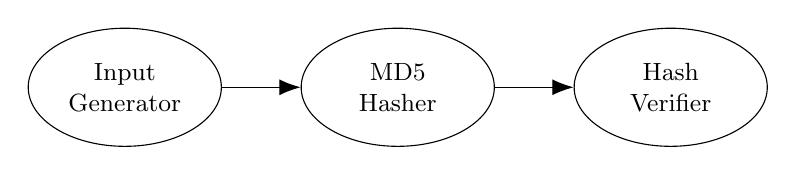
\begin{tikzpicture}[font=\small,
      rep style/.style={rectangle,draw=black,text width=1.5cm,minimum
        size=1.5cm,align=center},
      proc style/.style={ellipse,draw=black,align=center,text
        width=1.5cm,minimum size=1.5cm,align=center},
      file style/.style={ellipse,draw=none,align=center,text
        width=1.5cm,minimum size=0.5cm,align=center}
      ]

      \node[proc style] (gen) {Input\\Generator};
      \node[proc style, right=1cm of gen] (calc) {MD5 Hasher};
      \node[proc style, right=1cm of calc] (verify) {Hash\\Verifier};

      \draw[-{Latex[scale=1.6]}] (gen) edge  (calc);
      \draw[-{Latex[scale=1.6]}] (calc) edge  (verify);

    \end{tikzpicture}}
  \caption{Structure of the MD5 bruteforcer network.}
\end{figure}
\end{frame}

\begin{frame}
\begin{figure}%[tb]
\begin{minipage}{\linewidth}
  \centering
  \resizebox{.5\linewidth}{!}{
    \begin{tikzpicture}[font=\small,
      rep style/.style={rectangle,draw=black,text width=1.5cm,minimum
        size=1.5cm,align=center},
      proc style/.style={ellipse,draw=black,align=center,text
        width=1.5cm,minimum size=1.5cm,align=center},
      file style/.style={ellipse,draw=none,align=center,text
        width=1.5cm,minimum size=0.5cm,align=center},
      part/.pic={
        \node[] (m1) {\includegraphics[width=.10\textwidth]{../figures/7seg.pdf}};
        \node[left=0cm of m1] (m2) {\includegraphics[width=.10\textwidth]{../figures/7seg.pdf}};}
      ]

      \pic[local bounding box=hrs] {part};
      \node[below=2mm of hrs] (h2) {Hours};
      \pic[local bounding box=mins, right=30mm of hrs] {part};
      \node[below=2mm of mins] (m2) {Minutes};
      \pic[local bounding box=secs, right=30mm of mins] {part};
      \node[below=2mm of secs] (s2) {Seconds};

      \node[proc style, above=0.3cm of hrs] (dechrs) {Decoder};
      \node[proc style, above=0.3cm of mins] (decmins) {Decoder};
      \node[proc style, above=0.3cm of secs] (decsecs) {Decoder};

      \node[proc style, above=1cm of dechrs] (enchrs) {Encoder};
      \node[proc style, above=1cm of decmins] (encmins) {Encoder};
      \node[proc style, above=1cm of decsecs] (encsecs) {Encoder};
      
      \node[proc style, above=1cm of enchrs] (splithrs) {Calculate\\Hours};
      \node[proc style, above=1cm of encmins] (splitmins) {Calculate\\Minutes};
      \node[proc style, above=1cm of encsecs] (splitsecs) {Calculate\\Seconds};

      \draw[-{Latex[scale=1.6]}] (splithrs) edge (enchrs);
      \draw[-{Latex[scale=1.6]}] (splitmins) edge (encmins);
      \draw[-{Latex[scale=1.6]}] (splitsecs) edge (encsecs);

      \node[above=1cm of splitmins] (split) {};
      
      \node[proc style, above=2.5cm of split] (gen) {Timer};
      \draw[-] (gen) edge node [below left=0cm and 0cm of
      gen] {Seconds today} (split);

      \draw[-{Latex[scale=1.6]}] (split) edge (splithrs);
      \draw[-{Latex[scale=1.6]}] (split) edge (splitmins);
      \draw[-{Latex[scale=1.6]}] (split) edge (splitsecs);

      \draw[-{Latex[scale=1.6]}] (enchrs) edge (dechrs);
      \draw[-{Latex[scale=1.6]}] (encmins) edge (decmins);
      \draw[-{Latex[scale=1.6]}] (encsecs) edge (decsecs);

      \begin{scope}[on background layer]
        \node[draw=gray,inner sep=8pt,rounded corners=10pt,anchor=north
        west,fit=(enchrs)(encmins)(encsecs)(splithrs)(splitmins)(splitsecs)(gen),
        label={above}:Controller]
        (showhrs) {};
        \node[draw=gray,inner sep=8pt,rounded
        corners=10pt,anchor=north west,fit=(hrs)(dechrs)] (showhrs) {};
        \node[draw=gray,inner sep=8pt,rounded corners=10pt,anchor=north
        west,fit=(mins)(decmins)] (showmins) {}; \node[draw=gray,inner
        sep=8pt,rounded corners=10pt,anchor=north west,fit=(secs)(decsecs)]
        (showhrs) {};
      \end{scope}
    \end{tikzpicture}}
    \caption{Model digital clock using a 7-segment display. A timer keeps track
      of the number of seconds elapsed since midnight and several processes
      calculates and lights.}
\label{fig:7seg}
\end{minipage}
  \end{figure}
\end{frame}
\backupend

\end{document}

%%% Local Variables:
%%% mode: latex
%%% TeX-master: t
%%% TeX-command-extra-options: "-enable-write18"
%%% End:
